% Desktop-Bildschirm des WebTraders als schlichtes Lehrbuch-Schema (KEIN Nachbau, keine
% UI-Optik): Flächen und Linien in den Farbrollen des Pending-Orders-Guides (HANDOFF 13.1),
% Schrift IBM Plex Sans wie die Erklärgrafiken des Dokuments. Beschriftet sind nur die
% Bereiche (fett, ink) und Begriffe der Plattform (Regular, body/muted), ohne Zahlen,
% ohne Kurse, ohne Bid/Ask, ohne persönliche Angaben.
%
% Proportionen grob nach einem Screenshot des ganzen Desktop-Bildschirms (2000 x 969 px,
% blaues Design, nicht im Repo): Koordinaten unten in Pixeln dieses Screenshots,
% Ursprung oben links, y nach unten; 1 px = 0,085 mm -> 170 x 82,365 mm.
%   Kopfleiste       y 0–40          (nur angedeutet: Fläche ohne Inhalt)
%   Kursliste        x 0–317         Reiter All Quotes / Favorite, Kategorien; Metals
%                                    aufgeklappt (Zeilen ohne Namen, Info-Zeichen am Ende)
%   Chart            x 317–2000, y 40–658   SELL / BUY oben in der Mitte, Kurslinie
%   Tabelle der Positionen  y 658–917       Reiter Active / Pending / History rechts,
%                                    Auswahl der Spaltenköpfe (ohne S/L, T/P: kein Stop-Loss)
%   Unterste Leiste  y 917–969       Balance … Credit rechtsbündig, gleichmäßig verteilt
%                                    (Leiste etwas höher als im Screenshot: 52 statt 40 px)
%
% Kennbuchstaben A–D an den Bereichen (für eine spätere Legende), Standard: aus;
% mit Buchstaben bauen:  xelatex '\def\mitkennung{}% Desktop-Bildschirm des WebTraders als schlichtes Lehrbuch-Schema (KEIN Nachbau, keine
% UI-Optik): Flächen und Linien in den Farbrollen des Pending-Orders-Guides (HANDOFF 13.1),
% Schrift IBM Plex Sans wie die Erklärgrafiken des Dokuments. Beschriftet sind nur die
% Bereiche (fett, ink) und Begriffe der Plattform (Regular, body/muted), ohne Zahlen,
% ohne Kurse, ohne Bid/Ask, ohne persönliche Angaben.
%
% Proportionen grob nach einem Screenshot des ganzen Desktop-Bildschirms (2000 x 969 px,
% blaues Design, nicht im Repo): Koordinaten unten in Pixeln dieses Screenshots,
% Ursprung oben links, y nach unten; 1 px = 0,085 mm -> 170 x 82,365 mm.
%   Kopfleiste       y 0–40          (nur angedeutet: Fläche ohne Inhalt)
%   Kursliste        x 0–317         Reiter All Quotes / Favorite, Kategorien; Metals
%                                    aufgeklappt (Zeilen ohne Namen, Info-Zeichen am Ende)
%   Chart            x 317–2000, y 40–658   SELL / BUY oben in der Mitte, Kurslinie
%   Tabelle der Positionen  y 658–917       Reiter Active / Pending / History rechts,
%                                    Auswahl der Spaltenköpfe (ohne S/L, T/P: kein Stop-Loss)
%   Unterste Leiste  y 917–969       Balance … Credit rechtsbündig, gleichmäßig verteilt
%                                    (Leiste etwas höher als im Screenshot: 52 statt 40 px)
%
% Kennbuchstaben A–D an den Bereichen (für eine spätere Legende), Standard: aus;
% mit Buchstaben bauen:  xelatex '\def\mitkennung{}% Desktop-Bildschirm des WebTraders als schlichtes Lehrbuch-Schema (KEIN Nachbau, keine
% UI-Optik): Flächen und Linien in den Farbrollen des Pending-Orders-Guides (HANDOFF 13.1),
% Schrift IBM Plex Sans wie die Erklärgrafiken des Dokuments. Beschriftet sind nur die
% Bereiche (fett, ink) und Begriffe der Plattform (Regular, body/muted), ohne Zahlen,
% ohne Kurse, ohne Bid/Ask, ohne persönliche Angaben.
%
% Proportionen grob nach einem Screenshot des ganzen Desktop-Bildschirms (2000 x 969 px,
% blaues Design, nicht im Repo): Koordinaten unten in Pixeln dieses Screenshots,
% Ursprung oben links, y nach unten; 1 px = 0,085 mm -> 170 x 82,365 mm.
%   Kopfleiste       y 0–40          (nur angedeutet: Fläche ohne Inhalt)
%   Kursliste        x 0–317         Reiter All Quotes / Favorite, Kategorien; Metals
%                                    aufgeklappt (Zeilen ohne Namen, Info-Zeichen am Ende)
%   Chart            x 317–2000, y 40–658   SELL / BUY oben in der Mitte, Kurslinie
%   Tabelle der Positionen  y 658–917       Reiter Active / Pending / History rechts,
%                                    Auswahl der Spaltenköpfe (ohne S/L, T/P: kein Stop-Loss)
%   Unterste Leiste  y 917–969       Balance … Credit rechtsbündig, gleichmäßig verteilt
%                                    (Leiste etwas höher als im Screenshot: 52 statt 40 px)
%
% Kennbuchstaben A–D an den Bereichen (für eine spätere Legende), Standard: aus;
% mit Buchstaben bauen:  xelatex '\def\mitkennung{}% Desktop-Bildschirm des WebTraders als schlichtes Lehrbuch-Schema (KEIN Nachbau, keine
% UI-Optik): Flächen und Linien in den Farbrollen des Pending-Orders-Guides (HANDOFF 13.1),
% Schrift IBM Plex Sans wie die Erklärgrafiken des Dokuments. Beschriftet sind nur die
% Bereiche (fett, ink) und Begriffe der Plattform (Regular, body/muted), ohne Zahlen,
% ohne Kurse, ohne Bid/Ask, ohne persönliche Angaben.
%
% Proportionen grob nach einem Screenshot des ganzen Desktop-Bildschirms (2000 x 969 px,
% blaues Design, nicht im Repo): Koordinaten unten in Pixeln dieses Screenshots,
% Ursprung oben links, y nach unten; 1 px = 0,085 mm -> 170 x 82,365 mm.
%   Kopfleiste       y 0–40          (nur angedeutet: Fläche ohne Inhalt)
%   Kursliste        x 0–317         Reiter All Quotes / Favorite, Kategorien; Metals
%                                    aufgeklappt (Zeilen ohne Namen, Info-Zeichen am Ende)
%   Chart            x 317–2000, y 40–658   SELL / BUY oben in der Mitte, Kurslinie
%   Tabelle der Positionen  y 658–917       Reiter Active / Pending / History rechts,
%                                    Auswahl der Spaltenköpfe (ohne S/L, T/P: kein Stop-Loss)
%   Unterste Leiste  y 917–969       Balance … Credit rechtsbündig, gleichmäßig verteilt
%                                    (Leiste etwas höher als im Screenshot: 52 statt 40 px)
%
% Kennbuchstaben A–D an den Bereichen (für eine spätere Legende), Standard: aus;
% mit Buchstaben bauen:  xelatex '\def\mitkennung{}\input{desktop-schema.tex}'
\documentclass[border=0pt]{standalone}
\usepackage{fontspec}
\usepackage{tikz}
\usetikzlibrary{arrows.meta}
\setmainfont{IBMPlexSans-Regular.otf}[Path=../../fonts/,BoldFont={IBMPlexSans-SemiBold.otf}]

% Farben wie Kontogrundlagen-Kosten.tex (Rollen HANDOFF 13.1)
\definecolor{ink}{HTML}{14161A}    \definecolor{body}{HTML}{3C4249}
\definecolor{muted}{HTML}{6D757E}  \definecolor{rule}{HTML}{E2E5E9}
\definecolor{greya}{HTML}{A8AEB6}  \definecolor{paper}{HTML}{F7F8F9}
\definecolor{buy}{HTML}{0E7A4E}    \definecolor{sell}{HTML}{B23A2E}
\definecolor{buytint}{HTML}{E9F4EE} \definecolor{selltint}{HTML}{FAEDEB}
\definecolor{pfgrey}{HTML}{6A6A6A}

\newif\ifkennung \kennungfalse
\ifdefined\mitkennung \kennungtrue\fi

\newcommand\bereichf{\fontsize{8}{9.6}\selectfont\bfseries}% Name eines Bereichs
\newcommand\pf{\fontsize{6.3}{7.6}\selectfont}%             Begriff der Plattform
% Grundlinie: Mitte der Zeile + halbe Versalhöhe (Plex 0,698 em): 6,3 pt -> 9 px, 8 pt -> 11,5 px
\newcommand\begriff[4][body]{\node[anchor=base west,inner sep=0,font=\pf,text=#1] at (#2,#3+9) {#4};}
\newcommand\begriffm[4][body]{\node[anchor=base,inner sep=0,font=\pf,text=#1] at (#2,#3+9) {#4};}
% \bereich{name}{x}{y-Mitte}{Text}{Kennbuchstabe}
\newcommand\bereich[5]{\node[anchor=base west,inner sep=0,font=\bereichf,text=ink] (#1)
  at (#2,#3+11.5) {#4};%
  \ifkennung\node[circle,fill=ink,text=white,inner sep=0,minimum size=3.2mm,
    font=\bfseries\fontsize{5.6}{6}\selectfont] at ([xshift=2.6mm,yshift=0.99mm]#1.base east) {#5};\fi}

\begin{document}
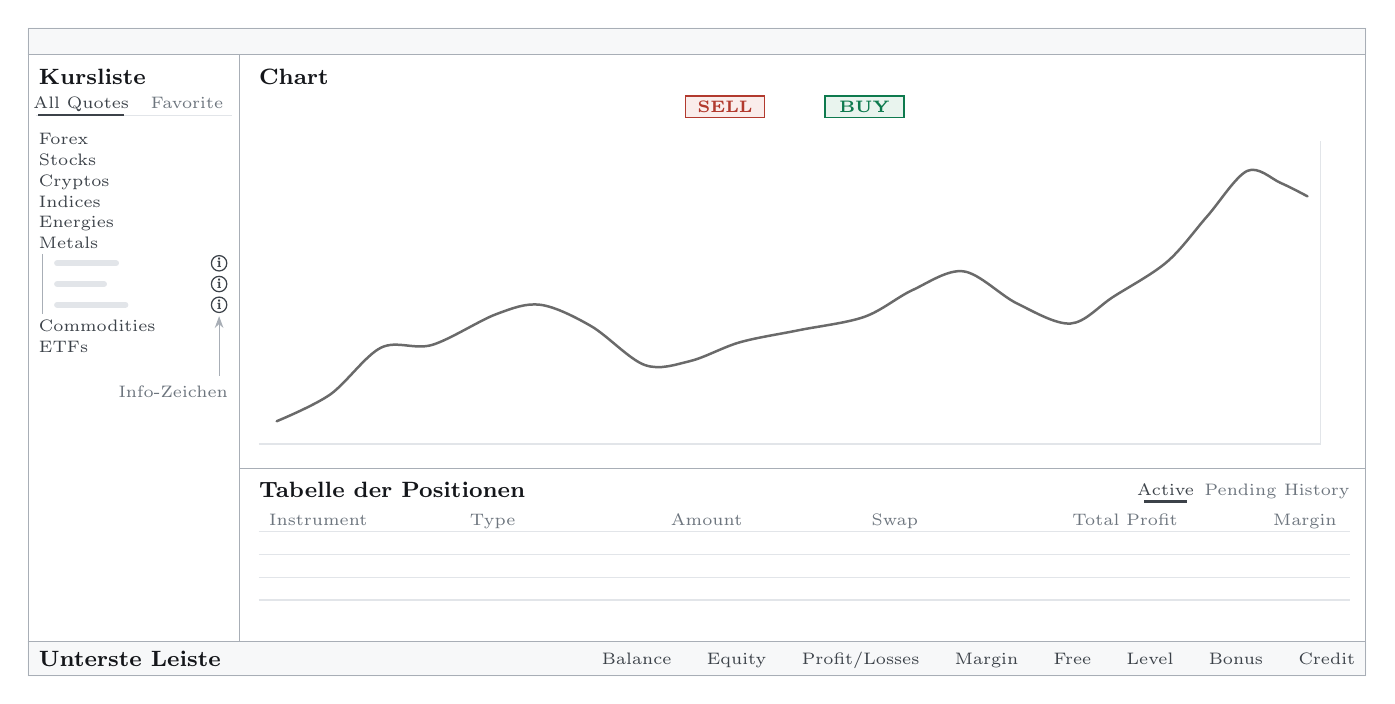
\begin{tikzpicture}[x=0.085mm,y=-0.085mm]
\useasboundingbox (0,0) rectangle (2000,969);
\tikzset{teilung/.style={greya,line width=0.4pt},
  fein/.style={rule,line width=0.4pt},
  platzhalter/.style={rule,line width=2.2pt,line cap=round}}

% ---- Gliederung: Kopfleiste und unterste Leiste getönt, Bereiche durch Linien getrennt
\fill[paper] (0,0) rectangle (2000,40) (0,917) rectangle (2000,969);
\draw[teilung] (0,40) -- (2000,40) (0,917) -- (2000,917)
  (317,40) -- (317,917) (317,658) -- (2000,658);
\draw[greya,line width=0.6pt]
  ([shift={(0.3pt,-0.3pt)}]0,0) rectangle ([shift={(-0.3pt,0.3pt)}]2000,969);

% ---- Kursliste ---------------------------------------------------------------
\bereich{nkurs}{16}{74}{Kursliste}{A}
\begriffm{80}{112}{All Quotes}
\begriffm[muted]{238}{112}{Favorite}
\draw[fein] (12,131) -- (305,131);
\draw[body,line width=0.8pt] (16,131) -- (144,131);
\foreach \y/\k in {166/Forex,197/Stocks,228/Cryptos,259/Indices,290/Energies,321/Metals,
  445/Commodities,476/ETFs} {\begriff{16}{\y}{\k}}
% aufgeklappte Kategorie: Zeilen der Instrumente (Name nur als Platzhalter), Info-Zeichen am Ende
\draw[greya,line width=0.4pt] (22,338) -- (22,428);
\foreach \y/\l in {352/132,383/114,414/146} {
  \draw[platzhalter] (44,\y) -- (\l,\y);
  \draw[body,line width=0.45pt] (286,\y) circle[radius=11.5];
  \node[inner sep=0,font=\bfseries\fontsize{5}{5}\selectfont,text=body] at (286,\y-0.5) {i};}
\draw[greya,line width=0.4pt,-{Stealth[length=1.5mm,width=1.1mm]}] (286,520) -- (286,431);
\node[anchor=base east,inner sep=0,font=\pf,text=muted] at (300,552) {Info-Zeichen};

% ---- Chart -------------------------------------------------------------------
\bereich{nchart}{345}{74}{Chart}{B}
\draw[sell,line width=0.5pt,fill=selltint] (983,102) rectangle (1101,134);
\node[inner sep=0,font=\pf\bfseries,text=sell] at (1042,118) {SELL};
\draw[buy,line width=0.5pt,fill=buytint] (1191,102) rectangle (1309,134);
\node[inner sep=0,font=\pf\bfseries,text=buy] at (1250,118) {BUY};
% Kurs- und Zeitskala als Haarlinien, Kurslinie neutral (Rolle der Kurslinie)
\draw[fein] (345,622) -- (1932,622) -- (1932,170);
\draw[pfgrey,line width=0.9pt,line join=round,line cap=round] plot[smooth,tension=0.55]
  coordinates {(372,588) (452,548) (528,478) (604,474) (700,428) (766,414) (842,446)
  (922,504) (990,498) (1064,470) (1152,452) (1250,432) (1322,392) (1398,364) (1478,412)
  (1558,442) (1622,402) (1702,350) (1762,282) (1822,214) (1872,232) (1912,252)};

% ---- Tabelle der Positionen --------------------------------------------------
\bereich{ntab}{345}{690}{Tabelle der Positionen}{C}
\begriffm{1700}{690}{Active}
\begriffm[muted]{1812}{690}{Pending}
\begriffm[muted]{1926}{690}{History}
\draw[body,line width=0.8pt] (1668,708) -- (1732,708);
\foreach \x/\k in {360/Instrument,660/Type,960/Amount,1260/Swap,1560/Total Profit,1860/Margin}
  {\begriff[muted]{\x}{735}{\k}}
\draw[fein] (345,753) -- (1975,753) (345,787) -- (1975,787) (345,821) -- (1975,821)
  (345,855) -- (1975,855);

% ---- Unterste Leiste ---------------------------------------------------------
\bereich{nleiste}{16}{943}{Unterste Leiste}{D}
% ohne Werte gleichmäßig verteilt, rechtsbündig wie im Original (dort ab etwa der Mitte)
\node[anchor=base east,inner sep=0,font=\pf,text=body] at (1984,943+9) {Balance\hspace{4.5mm}%
  Equity\hspace{4.5mm}Profit/Losses\hspace{4.5mm}Margin\hspace{4.5mm}Free\hspace{4.5mm}%
  Level\hspace{4.5mm}Bonus\hspace{4.5mm}Credit};
\end{tikzpicture}
\end{document}
'
\documentclass[border=0pt]{standalone}
\usepackage{fontspec}
\usepackage{tikz}
\usetikzlibrary{arrows.meta}
\setmainfont{IBMPlexSans-Regular.otf}[Path=../../fonts/,BoldFont={IBMPlexSans-SemiBold.otf}]

% Farben wie Kontogrundlagen-Kosten.tex (Rollen HANDOFF 13.1)
\definecolor{ink}{HTML}{14161A}    \definecolor{body}{HTML}{3C4249}
\definecolor{muted}{HTML}{6D757E}  \definecolor{rule}{HTML}{E2E5E9}
\definecolor{greya}{HTML}{A8AEB6}  \definecolor{paper}{HTML}{F7F8F9}
\definecolor{buy}{HTML}{0E7A4E}    \definecolor{sell}{HTML}{B23A2E}
\definecolor{buytint}{HTML}{E9F4EE} \definecolor{selltint}{HTML}{FAEDEB}
\definecolor{pfgrey}{HTML}{6A6A6A}

\newif\ifkennung \kennungfalse
\ifdefined\mitkennung \kennungtrue\fi

\newcommand\bereichf{\fontsize{8}{9.6}\selectfont\bfseries}% Name eines Bereichs
\newcommand\pf{\fontsize{6.3}{7.6}\selectfont}%             Begriff der Plattform
% Grundlinie: Mitte der Zeile + halbe Versalhöhe (Plex 0,698 em): 6,3 pt -> 9 px, 8 pt -> 11,5 px
\newcommand\begriff[4][body]{\node[anchor=base west,inner sep=0,font=\pf,text=#1] at (#2,#3+9) {#4};}
\newcommand\begriffm[4][body]{\node[anchor=base,inner sep=0,font=\pf,text=#1] at (#2,#3+9) {#4};}
% \bereich{name}{x}{y-Mitte}{Text}{Kennbuchstabe}
\newcommand\bereich[5]{\node[anchor=base west,inner sep=0,font=\bereichf,text=ink] (#1)
  at (#2,#3+11.5) {#4};%
  \ifkennung\node[circle,fill=ink,text=white,inner sep=0,minimum size=3.2mm,
    font=\bfseries\fontsize{5.6}{6}\selectfont] at ([xshift=2.6mm,yshift=0.99mm]#1.base east) {#5};\fi}

\begin{document}
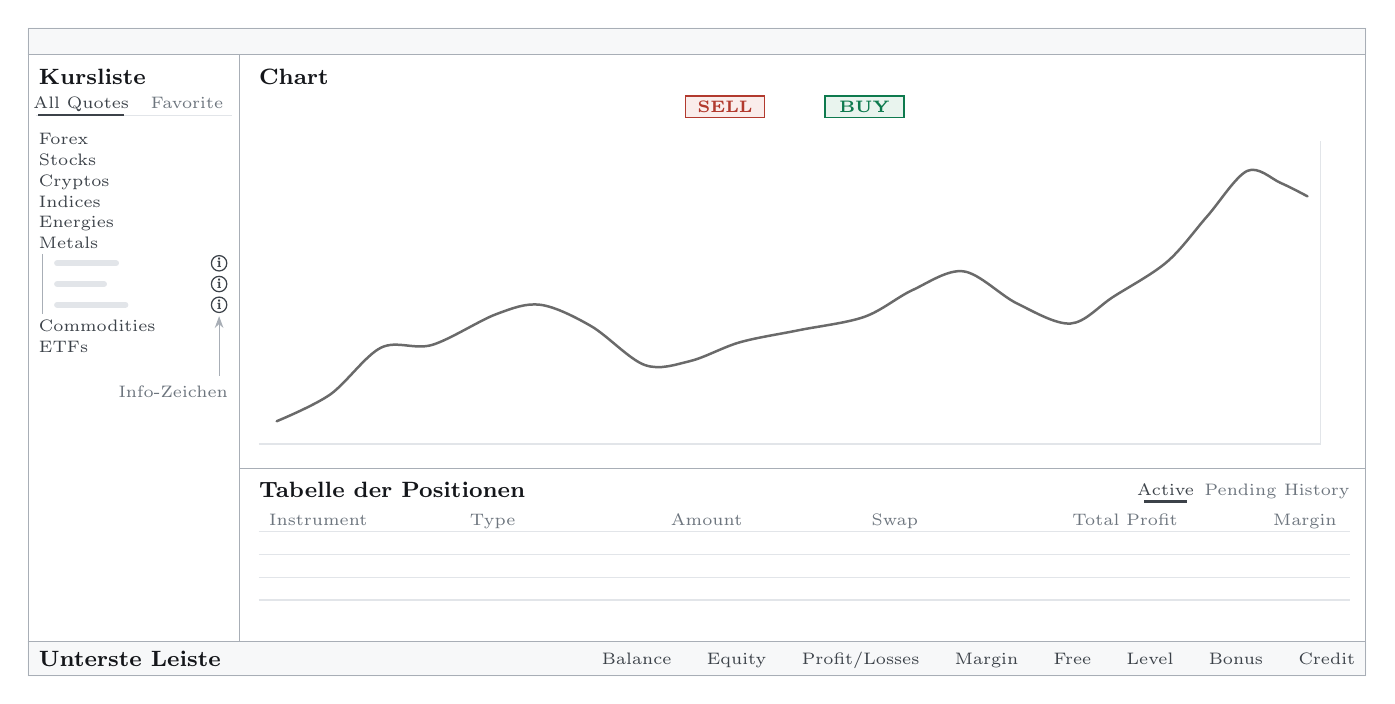
\begin{tikzpicture}[x=0.085mm,y=-0.085mm]
\useasboundingbox (0,0) rectangle (2000,969);
\tikzset{teilung/.style={greya,line width=0.4pt},
  fein/.style={rule,line width=0.4pt},
  platzhalter/.style={rule,line width=2.2pt,line cap=round}}

% ---- Gliederung: Kopfleiste und unterste Leiste getönt, Bereiche durch Linien getrennt
\fill[paper] (0,0) rectangle (2000,40) (0,917) rectangle (2000,969);
\draw[teilung] (0,40) -- (2000,40) (0,917) -- (2000,917)
  (317,40) -- (317,917) (317,658) -- (2000,658);
\draw[greya,line width=0.6pt]
  ([shift={(0.3pt,-0.3pt)}]0,0) rectangle ([shift={(-0.3pt,0.3pt)}]2000,969);

% ---- Kursliste ---------------------------------------------------------------
\bereich{nkurs}{16}{74}{Kursliste}{A}
\begriffm{80}{112}{All Quotes}
\begriffm[muted]{238}{112}{Favorite}
\draw[fein] (12,131) -- (305,131);
\draw[body,line width=0.8pt] (16,131) -- (144,131);
\foreach \y/\k in {166/Forex,197/Stocks,228/Cryptos,259/Indices,290/Energies,321/Metals,
  445/Commodities,476/ETFs} {\begriff{16}{\y}{\k}}
% aufgeklappte Kategorie: Zeilen der Instrumente (Name nur als Platzhalter), Info-Zeichen am Ende
\draw[greya,line width=0.4pt] (22,338) -- (22,428);
\foreach \y/\l in {352/132,383/114,414/146} {
  \draw[platzhalter] (44,\y) -- (\l,\y);
  \draw[body,line width=0.45pt] (286,\y) circle[radius=11.5];
  \node[inner sep=0,font=\bfseries\fontsize{5}{5}\selectfont,text=body] at (286,\y-0.5) {i};}
\draw[greya,line width=0.4pt,-{Stealth[length=1.5mm,width=1.1mm]}] (286,520) -- (286,431);
\node[anchor=base east,inner sep=0,font=\pf,text=muted] at (300,552) {Info-Zeichen};

% ---- Chart -------------------------------------------------------------------
\bereich{nchart}{345}{74}{Chart}{B}
\draw[sell,line width=0.5pt,fill=selltint] (983,102) rectangle (1101,134);
\node[inner sep=0,font=\pf\bfseries,text=sell] at (1042,118) {SELL};
\draw[buy,line width=0.5pt,fill=buytint] (1191,102) rectangle (1309,134);
\node[inner sep=0,font=\pf\bfseries,text=buy] at (1250,118) {BUY};
% Kurs- und Zeitskala als Haarlinien, Kurslinie neutral (Rolle der Kurslinie)
\draw[fein] (345,622) -- (1932,622) -- (1932,170);
\draw[pfgrey,line width=0.9pt,line join=round,line cap=round] plot[smooth,tension=0.55]
  coordinates {(372,588) (452,548) (528,478) (604,474) (700,428) (766,414) (842,446)
  (922,504) (990,498) (1064,470) (1152,452) (1250,432) (1322,392) (1398,364) (1478,412)
  (1558,442) (1622,402) (1702,350) (1762,282) (1822,214) (1872,232) (1912,252)};

% ---- Tabelle der Positionen --------------------------------------------------
\bereich{ntab}{345}{690}{Tabelle der Positionen}{C}
\begriffm{1700}{690}{Active}
\begriffm[muted]{1812}{690}{Pending}
\begriffm[muted]{1926}{690}{History}
\draw[body,line width=0.8pt] (1668,708) -- (1732,708);
\foreach \x/\k in {360/Instrument,660/Type,960/Amount,1260/Swap,1560/Total Profit,1860/Margin}
  {\begriff[muted]{\x}{735}{\k}}
\draw[fein] (345,753) -- (1975,753) (345,787) -- (1975,787) (345,821) -- (1975,821)
  (345,855) -- (1975,855);

% ---- Unterste Leiste ---------------------------------------------------------
\bereich{nleiste}{16}{943}{Unterste Leiste}{D}
% ohne Werte gleichmäßig verteilt, rechtsbündig wie im Original (dort ab etwa der Mitte)
\node[anchor=base east,inner sep=0,font=\pf,text=body] at (1984,943+9) {Balance\hspace{4.5mm}%
  Equity\hspace{4.5mm}Profit/Losses\hspace{4.5mm}Margin\hspace{4.5mm}Free\hspace{4.5mm}%
  Level\hspace{4.5mm}Bonus\hspace{4.5mm}Credit};
\end{tikzpicture}
\end{document}
'
\documentclass[border=0pt]{standalone}
\usepackage{fontspec}
\usepackage{tikz}
\usetikzlibrary{arrows.meta}
\setmainfont{IBMPlexSans-Regular.otf}[Path=../../fonts/,BoldFont={IBMPlexSans-SemiBold.otf}]

% Farben wie Kontogrundlagen-Kosten.tex (Rollen HANDOFF 13.1)
\definecolor{ink}{HTML}{14161A}    \definecolor{body}{HTML}{3C4249}
\definecolor{muted}{HTML}{6D757E}  \definecolor{rule}{HTML}{E2E5E9}
\definecolor{greya}{HTML}{A8AEB6}  \definecolor{paper}{HTML}{F7F8F9}
\definecolor{buy}{HTML}{0E7A4E}    \definecolor{sell}{HTML}{B23A2E}
\definecolor{buytint}{HTML}{E9F4EE} \definecolor{selltint}{HTML}{FAEDEB}
\definecolor{pfgrey}{HTML}{6A6A6A}

\newif\ifkennung \kennungfalse
\ifdefined\mitkennung \kennungtrue\fi

\newcommand\bereichf{\fontsize{8}{9.6}\selectfont\bfseries}% Name eines Bereichs
\newcommand\pf{\fontsize{6.3}{7.6}\selectfont}%             Begriff der Plattform
% Grundlinie: Mitte der Zeile + halbe Versalhöhe (Plex 0,698 em): 6,3 pt -> 9 px, 8 pt -> 11,5 px
\newcommand\begriff[4][body]{\node[anchor=base west,inner sep=0,font=\pf,text=#1] at (#2,#3+9) {#4};}
\newcommand\begriffm[4][body]{\node[anchor=base,inner sep=0,font=\pf,text=#1] at (#2,#3+9) {#4};}
% \bereich{name}{x}{y-Mitte}{Text}{Kennbuchstabe}
\newcommand\bereich[5]{\node[anchor=base west,inner sep=0,font=\bereichf,text=ink] (#1)
  at (#2,#3+11.5) {#4};%
  \ifkennung\node[circle,fill=ink,text=white,inner sep=0,minimum size=3.2mm,
    font=\bfseries\fontsize{5.6}{6}\selectfont] at ([xshift=2.6mm,yshift=0.99mm]#1.base east) {#5};\fi}

\begin{document}
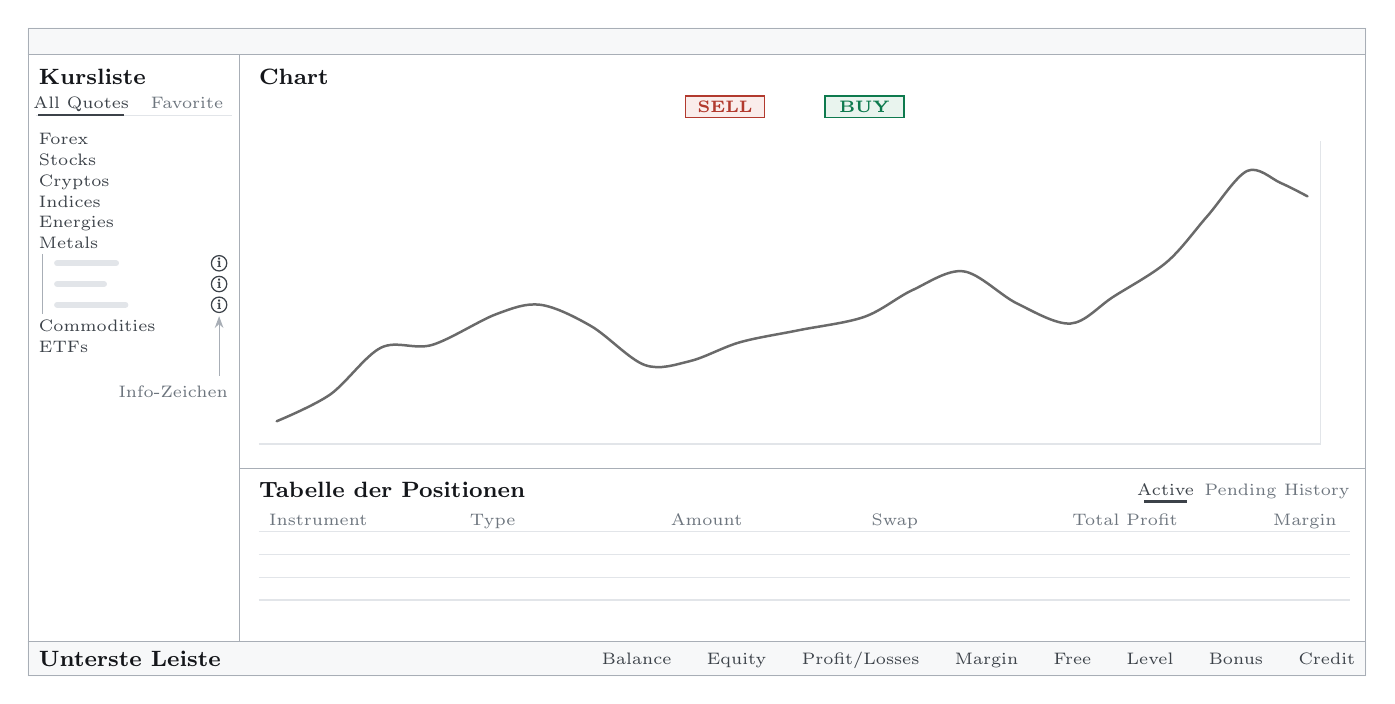
\begin{tikzpicture}[x=0.085mm,y=-0.085mm]
\useasboundingbox (0,0) rectangle (2000,969);
\tikzset{teilung/.style={greya,line width=0.4pt},
  fein/.style={rule,line width=0.4pt},
  platzhalter/.style={rule,line width=2.2pt,line cap=round}}

% ---- Gliederung: Kopfleiste und unterste Leiste getönt, Bereiche durch Linien getrennt
\fill[paper] (0,0) rectangle (2000,40) (0,917) rectangle (2000,969);
\draw[teilung] (0,40) -- (2000,40) (0,917) -- (2000,917)
  (317,40) -- (317,917) (317,658) -- (2000,658);
\draw[greya,line width=0.6pt]
  ([shift={(0.3pt,-0.3pt)}]0,0) rectangle ([shift={(-0.3pt,0.3pt)}]2000,969);

% ---- Kursliste ---------------------------------------------------------------
\bereich{nkurs}{16}{74}{Kursliste}{A}
\begriffm{80}{112}{All Quotes}
\begriffm[muted]{238}{112}{Favorite}
\draw[fein] (12,131) -- (305,131);
\draw[body,line width=0.8pt] (16,131) -- (144,131);
\foreach \y/\k in {166/Forex,197/Stocks,228/Cryptos,259/Indices,290/Energies,321/Metals,
  445/Commodities,476/ETFs} {\begriff{16}{\y}{\k}}
% aufgeklappte Kategorie: Zeilen der Instrumente (Name nur als Platzhalter), Info-Zeichen am Ende
\draw[greya,line width=0.4pt] (22,338) -- (22,428);
\foreach \y/\l in {352/132,383/114,414/146} {
  \draw[platzhalter] (44,\y) -- (\l,\y);
  \draw[body,line width=0.45pt] (286,\y) circle[radius=11.5];
  \node[inner sep=0,font=\bfseries\fontsize{5}{5}\selectfont,text=body] at (286,\y-0.5) {i};}
\draw[greya,line width=0.4pt,-{Stealth[length=1.5mm,width=1.1mm]}] (286,520) -- (286,431);
\node[anchor=base east,inner sep=0,font=\pf,text=muted] at (300,552) {Info-Zeichen};

% ---- Chart -------------------------------------------------------------------
\bereich{nchart}{345}{74}{Chart}{B}
\draw[sell,line width=0.5pt,fill=selltint] (983,102) rectangle (1101,134);
\node[inner sep=0,font=\pf\bfseries,text=sell] at (1042,118) {SELL};
\draw[buy,line width=0.5pt,fill=buytint] (1191,102) rectangle (1309,134);
\node[inner sep=0,font=\pf\bfseries,text=buy] at (1250,118) {BUY};
% Kurs- und Zeitskala als Haarlinien, Kurslinie neutral (Rolle der Kurslinie)
\draw[fein] (345,622) -- (1932,622) -- (1932,170);
\draw[pfgrey,line width=0.9pt,line join=round,line cap=round] plot[smooth,tension=0.55]
  coordinates {(372,588) (452,548) (528,478) (604,474) (700,428) (766,414) (842,446)
  (922,504) (990,498) (1064,470) (1152,452) (1250,432) (1322,392) (1398,364) (1478,412)
  (1558,442) (1622,402) (1702,350) (1762,282) (1822,214) (1872,232) (1912,252)};

% ---- Tabelle der Positionen --------------------------------------------------
\bereich{ntab}{345}{690}{Tabelle der Positionen}{C}
\begriffm{1700}{690}{Active}
\begriffm[muted]{1812}{690}{Pending}
\begriffm[muted]{1926}{690}{History}
\draw[body,line width=0.8pt] (1668,708) -- (1732,708);
\foreach \x/\k in {360/Instrument,660/Type,960/Amount,1260/Swap,1560/Total Profit,1860/Margin}
  {\begriff[muted]{\x}{735}{\k}}
\draw[fein] (345,753) -- (1975,753) (345,787) -- (1975,787) (345,821) -- (1975,821)
  (345,855) -- (1975,855);

% ---- Unterste Leiste ---------------------------------------------------------
\bereich{nleiste}{16}{943}{Unterste Leiste}{D}
% ohne Werte gleichmäßig verteilt, rechtsbündig wie im Original (dort ab etwa der Mitte)
\node[anchor=base east,inner sep=0,font=\pf,text=body] at (1984,943+9) {Balance\hspace{4.5mm}%
  Equity\hspace{4.5mm}Profit/Losses\hspace{4.5mm}Margin\hspace{4.5mm}Free\hspace{4.5mm}%
  Level\hspace{4.5mm}Bonus\hspace{4.5mm}Credit};
\end{tikzpicture}
\end{document}
'
\documentclass[border=0pt]{standalone}
\usepackage{fontspec}
\usepackage{tikz}
\usetikzlibrary{arrows.meta}
\setmainfont{IBMPlexSans-Regular.otf}[Path=../../fonts/,BoldFont={IBMPlexSans-SemiBold.otf}]

% Farben wie Kontogrundlagen-Kosten.tex (Rollen HANDOFF 13.1)
\definecolor{ink}{HTML}{14161A}    \definecolor{body}{HTML}{3C4249}
\definecolor{muted}{HTML}{6D757E}  \definecolor{rule}{HTML}{E2E5E9}
\definecolor{greya}{HTML}{A8AEB6}  \definecolor{paper}{HTML}{F7F8F9}
\definecolor{buy}{HTML}{0E7A4E}    \definecolor{sell}{HTML}{B23A2E}
\definecolor{buytint}{HTML}{E9F4EE} \definecolor{selltint}{HTML}{FAEDEB}
\definecolor{pfgrey}{HTML}{6A6A6A}

\newif\ifkennung \kennungfalse
\ifdefined\mitkennung \kennungtrue\fi

\newcommand\bereichf{\fontsize{8}{9.6}\selectfont\bfseries}% Name eines Bereichs
\newcommand\pf{\fontsize{6.3}{7.6}\selectfont}%             Begriff der Plattform
% Grundlinie: Mitte der Zeile + halbe Versalhöhe (Plex 0,698 em): 6,3 pt -> 9 px, 8 pt -> 11,5 px
\newcommand\begriff[4][body]{\node[anchor=base west,inner sep=0,font=\pf,text=#1] at (#2,#3+9) {#4};}
\newcommand\begriffm[4][body]{\node[anchor=base,inner sep=0,font=\pf,text=#1] at (#2,#3+9) {#4};}
% \bereich{name}{x}{y-Mitte}{Text}{Kennbuchstabe}
\newcommand\bereich[5]{\node[anchor=base west,inner sep=0,font=\bereichf,text=ink] (#1)
  at (#2,#3+11.5) {#4};%
  \ifkennung\node[circle,fill=ink,text=white,inner sep=0,minimum size=3.2mm,
    font=\bfseries\fontsize{5.6}{6}\selectfont] at ([xshift=2.6mm,yshift=0.99mm]#1.base east) {#5};\fi}

\begin{document}
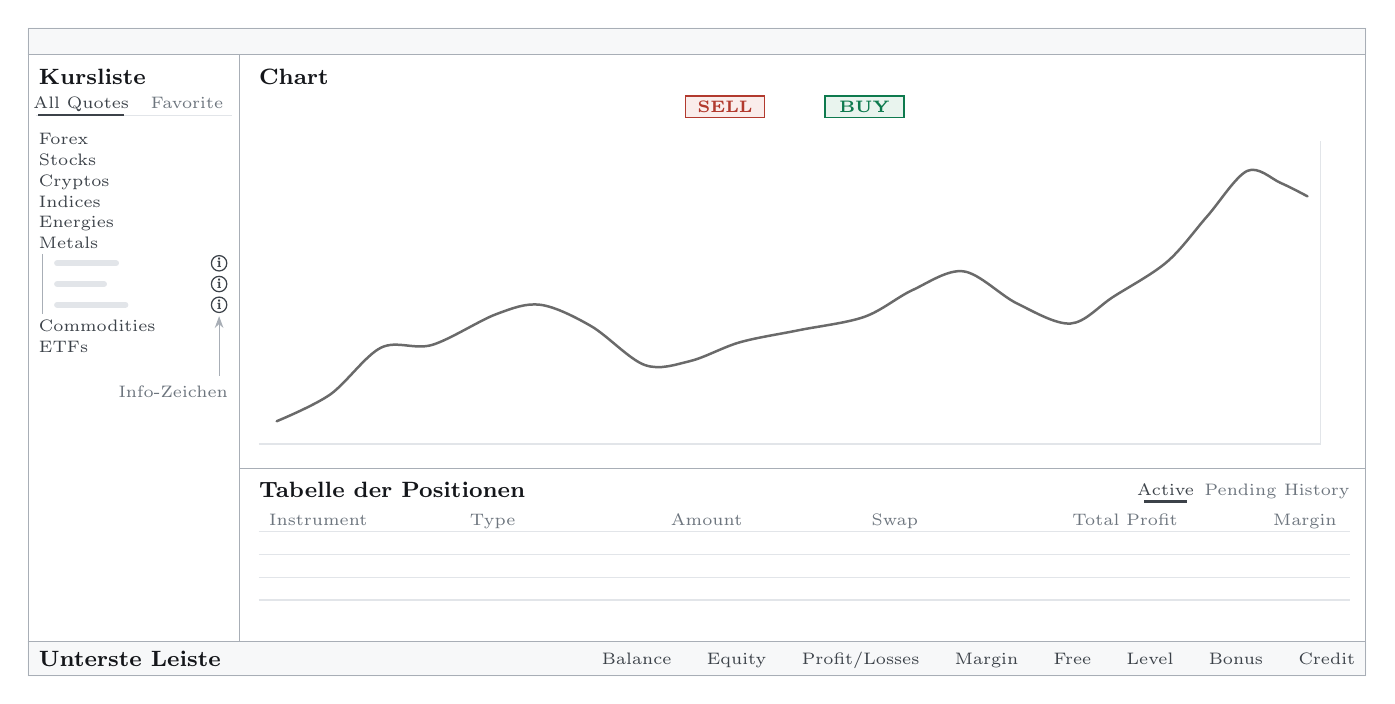
\begin{tikzpicture}[x=0.085mm,y=-0.085mm]
\useasboundingbox (0,0) rectangle (2000,969);
\tikzset{teilung/.style={greya,line width=0.4pt},
  fein/.style={rule,line width=0.4pt},
  platzhalter/.style={rule,line width=2.2pt,line cap=round}}

% ---- Gliederung: Kopfleiste und unterste Leiste getönt, Bereiche durch Linien getrennt
\fill[paper] (0,0) rectangle (2000,40) (0,917) rectangle (2000,969);
\draw[teilung] (0,40) -- (2000,40) (0,917) -- (2000,917)
  (317,40) -- (317,917) (317,658) -- (2000,658);
\draw[greya,line width=0.6pt]
  ([shift={(0.3pt,-0.3pt)}]0,0) rectangle ([shift={(-0.3pt,0.3pt)}]2000,969);

% ---- Kursliste ---------------------------------------------------------------
\bereich{nkurs}{16}{74}{Kursliste}{A}
\begriffm{80}{112}{All Quotes}
\begriffm[muted]{238}{112}{Favorite}
\draw[fein] (12,131) -- (305,131);
\draw[body,line width=0.8pt] (16,131) -- (144,131);
\foreach \y/\k in {166/Forex,197/Stocks,228/Cryptos,259/Indices,290/Energies,321/Metals,
  445/Commodities,476/ETFs} {\begriff{16}{\y}{\k}}
% aufgeklappte Kategorie: Zeilen der Instrumente (Name nur als Platzhalter), Info-Zeichen am Ende
\draw[greya,line width=0.4pt] (22,338) -- (22,428);
\foreach \y/\l in {352/132,383/114,414/146} {
  \draw[platzhalter] (44,\y) -- (\l,\y);
  \draw[body,line width=0.45pt] (286,\y) circle[radius=11.5];
  \node[inner sep=0,font=\bfseries\fontsize{5}{5}\selectfont,text=body] at (286,\y-0.5) {i};}
\draw[greya,line width=0.4pt,-{Stealth[length=1.5mm,width=1.1mm]}] (286,520) -- (286,431);
\node[anchor=base east,inner sep=0,font=\pf,text=muted] at (300,552) {Info-Zeichen};

% ---- Chart -------------------------------------------------------------------
\bereich{nchart}{345}{74}{Chart}{B}
\draw[sell,line width=0.5pt,fill=selltint] (983,102) rectangle (1101,134);
\node[inner sep=0,font=\pf\bfseries,text=sell] at (1042,118) {SELL};
\draw[buy,line width=0.5pt,fill=buytint] (1191,102) rectangle (1309,134);
\node[inner sep=0,font=\pf\bfseries,text=buy] at (1250,118) {BUY};
% Kurs- und Zeitskala als Haarlinien, Kurslinie neutral (Rolle der Kurslinie)
\draw[fein] (345,622) -- (1932,622) -- (1932,170);
\draw[pfgrey,line width=0.9pt,line join=round,line cap=round] plot[smooth,tension=0.55]
  coordinates {(372,588) (452,548) (528,478) (604,474) (700,428) (766,414) (842,446)
  (922,504) (990,498) (1064,470) (1152,452) (1250,432) (1322,392) (1398,364) (1478,412)
  (1558,442) (1622,402) (1702,350) (1762,282) (1822,214) (1872,232) (1912,252)};

% ---- Tabelle der Positionen --------------------------------------------------
\bereich{ntab}{345}{690}{Tabelle der Positionen}{C}
\begriffm{1700}{690}{Active}
\begriffm[muted]{1812}{690}{Pending}
\begriffm[muted]{1926}{690}{History}
\draw[body,line width=0.8pt] (1668,708) -- (1732,708);
\foreach \x/\k in {360/Instrument,660/Type,960/Amount,1260/Swap,1560/Total Profit,1860/Margin}
  {\begriff[muted]{\x}{735}{\k}}
\draw[fein] (345,753) -- (1975,753) (345,787) -- (1975,787) (345,821) -- (1975,821)
  (345,855) -- (1975,855);

% ---- Unterste Leiste ---------------------------------------------------------
\bereich{nleiste}{16}{943}{Unterste Leiste}{D}
% ohne Werte gleichmäßig verteilt, rechtsbündig wie im Original (dort ab etwa der Mitte)
\node[anchor=base east,inner sep=0,font=\pf,text=body] at (1984,943+9) {Balance\hspace{4.5mm}%
  Equity\hspace{4.5mm}Profit/Losses\hspace{4.5mm}Margin\hspace{4.5mm}Free\hspace{4.5mm}%
  Level\hspace{4.5mm}Bonus\hspace{4.5mm}Credit};
\end{tikzpicture}
\end{document}
